\chapter{Implementation}
\label{chap:implementation}
In this chapter, the implementation of the network stack using the
pipelined design from chapter \ref{chap:design} is outlined and described,
the application of SME detailed and evaluated, and lastly, the viability
of the system on an FPGA is discussed.\\
The network stack is implemented in C\# using the C\# version of SME, which is,
at the moment of writing, more mature and feature-rich. The current version of
the implementation supports most of the absolutely vital parts of the IPv4
protocol, as well as the UDP protocol, as specified by RFC 1122\cite{RFC1122}.
Although work has been carried out in order to ensure that additional protocols
can be implemented without obstructions, no additional protocols are supported
at the moment.\\
The solution is fairly well-divided into 3 different types of components,
relating closely to those of SME: processes, buffers, and busses. The most
interesting parts of these components will be described in further detail in the
following sections.


\section{Processes}
The processes are arguably the most vital part of the system, as they provide
the computation and "processing" on the in- and out-going packets.
It is important to note that although there are many other types of "processes",
in the network, such as the buffers, we will mainly refer to the modules doing
actual business-logic as "processes" \footnote{These processes are not to be
confused with SME processes, which are used for the implementation of both the
buffers and processes.}.

The essential processes in the network are represented as light-grey boxes in
the figure \ref{fig:final_design}. These processes are \texttt{Internet\_In},
\texttt{Internet\_Out}, and \texttt{Transport}.


\subsection{State-machines}
Network communication can consists of countless different packets, formats,
protocols, combinations of flags and settings, and even errors and corrupted
bits. The processes in the network have to take on a manifold of jobs in order
to handle all these scenarios, which sadly cannot be handled with a simple
combinational logic circuit. To operate under these various conditions, these
processes are modelled as finite state machines, maintaining a single state at
all times.\\
The processes have a lot of similar states, such as \texttt{Idle}, \texttt{Receive},
\texttt{Pass}, or \texttt{Send}, but these can work very differently, as shown
in the following sections. Before moving on to describing the state-machines of
the 3 processes, it is crucial to understand how these can be modelled in SME.

\subsubsection{SME process execution flow}
To implement a process in SME, the C\# class has to inherit from
either the \texttt{Process} abstract class, or the more simple
\texttt{SimpleProcess} class.
The latter class is, as its name states, a simpler version of the former. This
class implements an \texttt{OnTick()} method, which is invoked once for every
clock-cycle.\\
The more advanced, but also more capable \texttt{Process} class provides
an abstract method \texttt{Run} which is to be overriden and filled
with the code desired to be run in the process. The interesting feature
about this method is that it is asynchronous, meaning that the code can
execute other tasks while waiting for resources, such as functions,
to return. In this case, this asynchronous feature is used to give
the programmer ability to split the function into multiple segments,
separated by the clock signal.\\
Figure \ref{fig:example_fsm} compares these two approaches for the same
finite state-machine with 3 consequtive states.

The "synchronous" approach using a \texttt{SimpleProcess} in subfigure
\ref{fig:sme_example_process_sync_code} has to implement a
variable tracking the current state of the process. On each new clock, this
state has to be analysed and the inteded function to be called based on the
value. This approach requires a lot of approach and boilerplate code, especialy
if there are several states.\\
The asynchronous approach on subfigure
\ref{sme_example_process_async_code} on the other hand can do with only
single \texttt{Run()} method split into three parts -- A, B, and C.
After each code-segment, the process waits for the clock signal, and
continues with the execution of the next segment.  This functionality
gives the programmer a very granular control of the way a process
works, how it is split into multiple steps on the hardware, while
maintaining simplicity, as seen on the statemachine diagram on subfigure
\ref{fig:sme_example_process_fsm}.

\begin{figure*}[b]
    \begin{subfigure}[b]{0.3\textwidth}
        \centering
\begin{lstlisting}[language={[Sharp]C}]
public class SomeProcess : Process
{
  private override async Task Run()
  {
    // A
    await ClockAsync();
    // B
    await ClockAsync();
    // C
    await ClockAsync();
  }
}
\end{lstlisting}
        \caption{Example using inheriting from \texttt{Process}, using the \texttt{Run()} asynchronous method.}
	\label{fig:sme_example_process_async_code}
    \end{subfigure}
\hfill
    \begin{subfigure}[b]{0.3\textwidth}
\begin{lstlisting}[language={[Sharp]C}]
public class SomeProcess : SimpleProcess
{
// Initial state
state = A;

protected override void OnTick()
{
  switch(state) {
    case A:
      a();
      state = B;
    case B:
      b();
      state = C;
    case C:
      c();
      state = A;
  }

}
\end{lstlisting}
	\caption{Example pseudocode of using a "synchronous" \texttt{SimpleProcess}}
	\label{fig:sme_example_process_sync_code}
    \end{subfigure}
\hfill
 \begin{subfigure}[b]{0.3\textwidth}
        \centering
        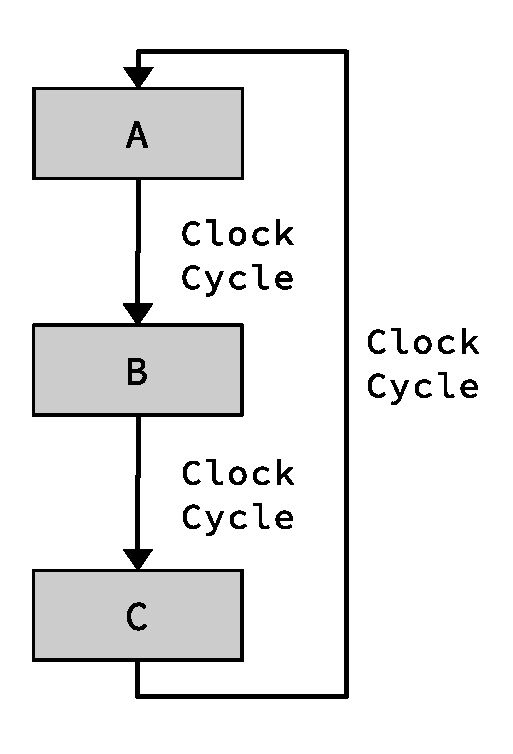
\includegraphics[scale=0.45]{implementation/empty_process_fsm.eps}
        \caption{The statemachine resulting from both code-examples}
 	\label{fig:sme_example_process_fsm}
\end{subfigure}
    \caption{A simple state-machine implemented in the asynchronous (left) and
asynchronous (right) approach in SME using C\#}
    \label{fig:example_fsm}
\end{figure*}


\subsubsection{\texttt{Internet Out} state machine}
This way of modelling a process in SME first the \texttt{Internet Out} process
very well, as it only has one responsibility, which is reading outgoing segments
and wrapping them in an Internet header. The figure \ref{fig:internet_out_implementation} shows the pseudo-code and state-machine for the \texttt{Internet Out}
process. This process was easy to model and implement, because it only has one
input and one output, and the state-changes are simple and intuitive.

\begin{figure*}[htpb]
    \centering
    \begin{subfigure}[b]{0.5\textwidth}
        \centering
\begin{lstlisting}[language={[Sharp]C}]
public partial class InternetOut: Process
{
public override async Task Run()
{
  while segment_available() {
    pass_segment();
    await ClockAsync();
  }

  while header_available() {
    pass_header();
    await ClockAsync();
  }
}
}
\end{lstlisting}
        \caption{Pseudo-code for the \texttt{InternetOut} process}
	\label{fig:internet_out_pseudocode}
    \end{subfigure}%
    \begin{subfigure}[b]{0.50\textwidth}
        \centering
        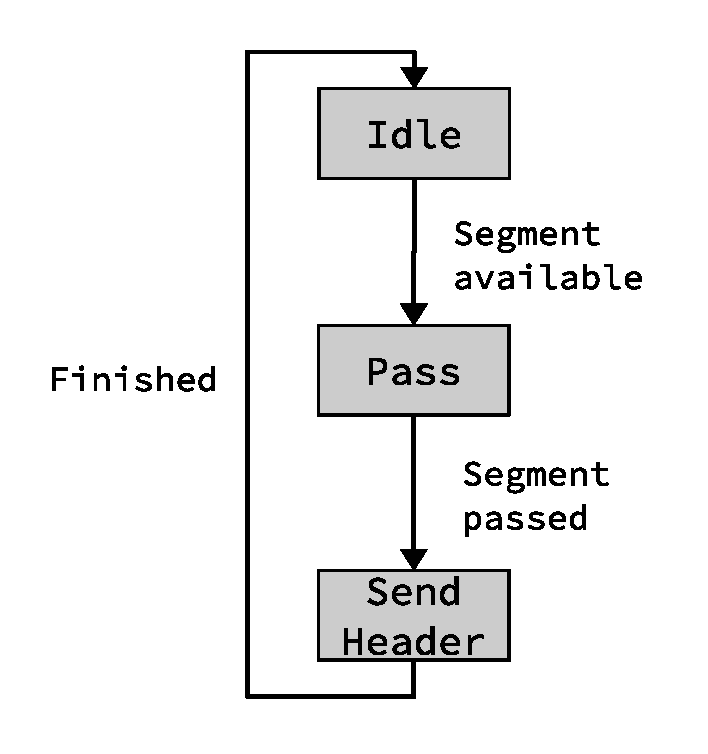
\includegraphics[scale=0.45]{implementation/internet_out_fsm.eps}
        \caption{The statemachine for the \texttt{InternetOut} process}
 	\label{fig:internet_out_fsm}
    \end{subfigure}%
    \caption{The implementation of the \texttt{InternetOut} process}
    \label{fig:internet_out_implementation}
\end{figure*}


\subsubsection{\texttt{Internet In} and \texttt{Transport} state machines}
Unfortunately,
The state-machine of \texttt{Internet In} is probably the most simple of all the
state-machines, as it can effectively only read new packets from the Link-layer,
and pass it along the pipeline. Although it might be desireable for the Internet
layer to send control packets out to the network, this is not supported in the
current build.


\begin{figure*}[t!]
    \centering
    \begin{subfigure}[t]{0.5\textwidth}
        \centering
        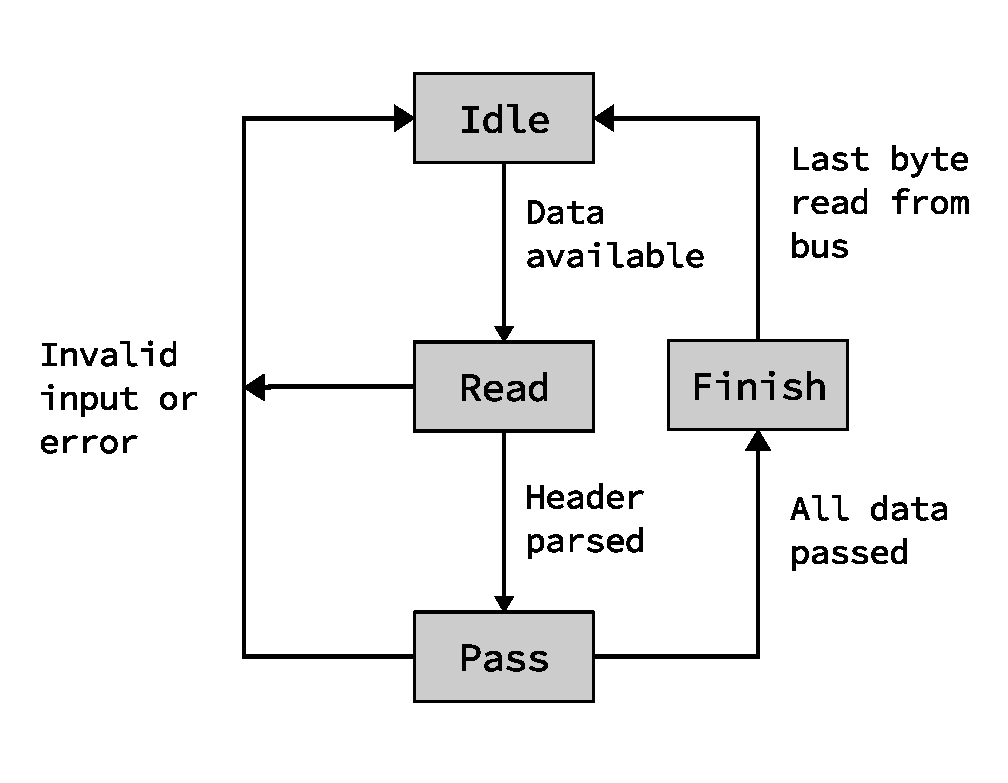
\includegraphics[scale=0.45]{implementation/internet_in_fsm.eps}
        \caption{The \texttt{Internet In} state machine}
    \end{subfigure}%
    ~
    \begin{subfigure}[t]{0.5\textwidth}
        \centering
        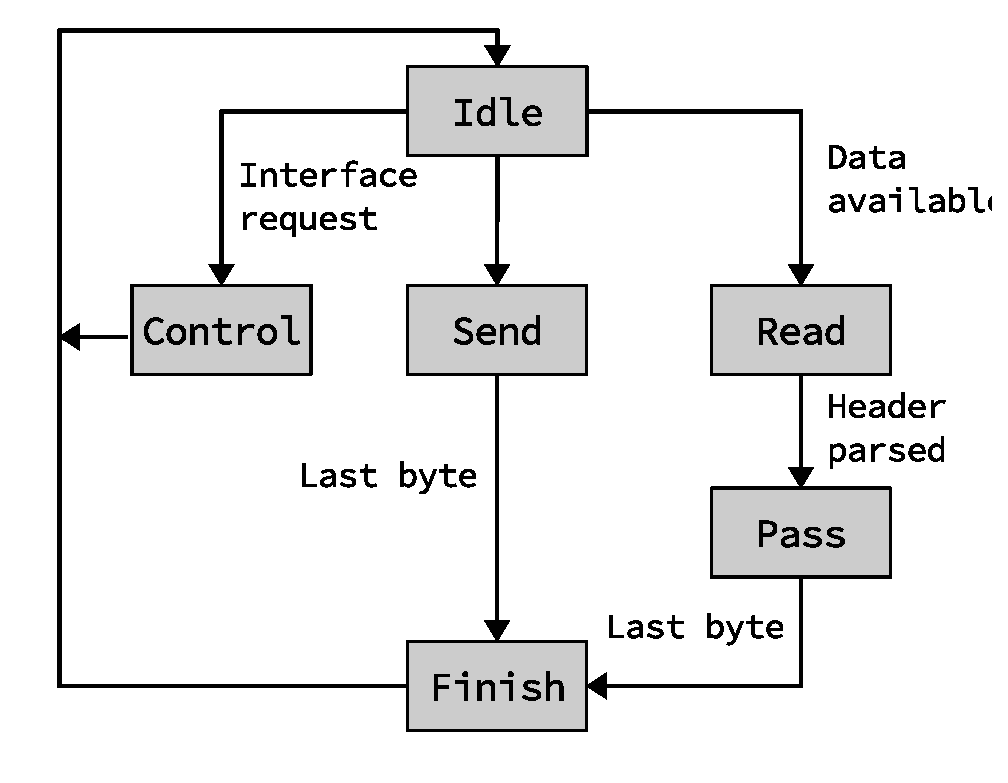
\includegraphics[scale=0.45]{implementation/transport_fsm.eps}
        \caption{The \texttt{Transport} state machine}
    \end{subfigure}%

    \caption{Statemachines for \texttt{Internet In} and \texttt{Transport}}
\end{figure*}

\subsubsection{\texttt{Internet Out} state machine}


\subsection{Internal memory}


\section{Buffers}
\subsection{Internal memory}
\subsection{IPv4 de-fragmentation and segment unification}
\subsection{Allocation}


\section{Busses}
\section{Interface Signal protocols}
\label{sec:interface_signal_protocol}
With the introduction of buffers between each parsing processes, a clear pattern
emerged. The layer-handling processes are responsible for numerous real-time tasks
(parsing, sending, protocol-specific tasks, etc), while also limited by their
fixed internal buffers. These processes are not always ready to receive input
from preceding processes, while they at the same time must be able to write their
output to following processes immediatelly.\\
The buffers are a stark opposite, as their large internal block memories enable
them to buffer huge chunks of memory, while also being able to wait for the
succeeding process to start reading.\\
With these two established scenarios, protocols for each can be proposed.

\subsection{Buffer-Producer}
\subsection{Compute-Producer}



\section{Interface Control}
\subsection{Usage}
\subsection{Limitations}

